\subsectionA{Pterran}
Pterrans are 1.5 to 1.9 meters tall reptiles with light brown scaly skin, sharp teeth, and a short tail. Pterrans wear little clothing, preferring belts and loincloths, or sashes. They walk upright, like humanoids, and have opposing thumbs and three-fingered, talon-clawed hands. Pterrans have two shoulder stumps, remnants of wings they possessed long ago, and a finlike growth juts out at the back of their heads. Pterrans weigh between 90 to 110 kilograms. There is no visible distinction between male and female pterrans.

Pterrans are rarely seen in the Tablelands. They live their lives in the Hinterlands, rarely leaving the safety of their villages. However, the recent earthquake and subsequent storms have brought disruption into the pterran's lives. More pterrans now venture outside their homes, and come to the Tyr region to seek trade and information.

\begin{figure}[t!]
\centering
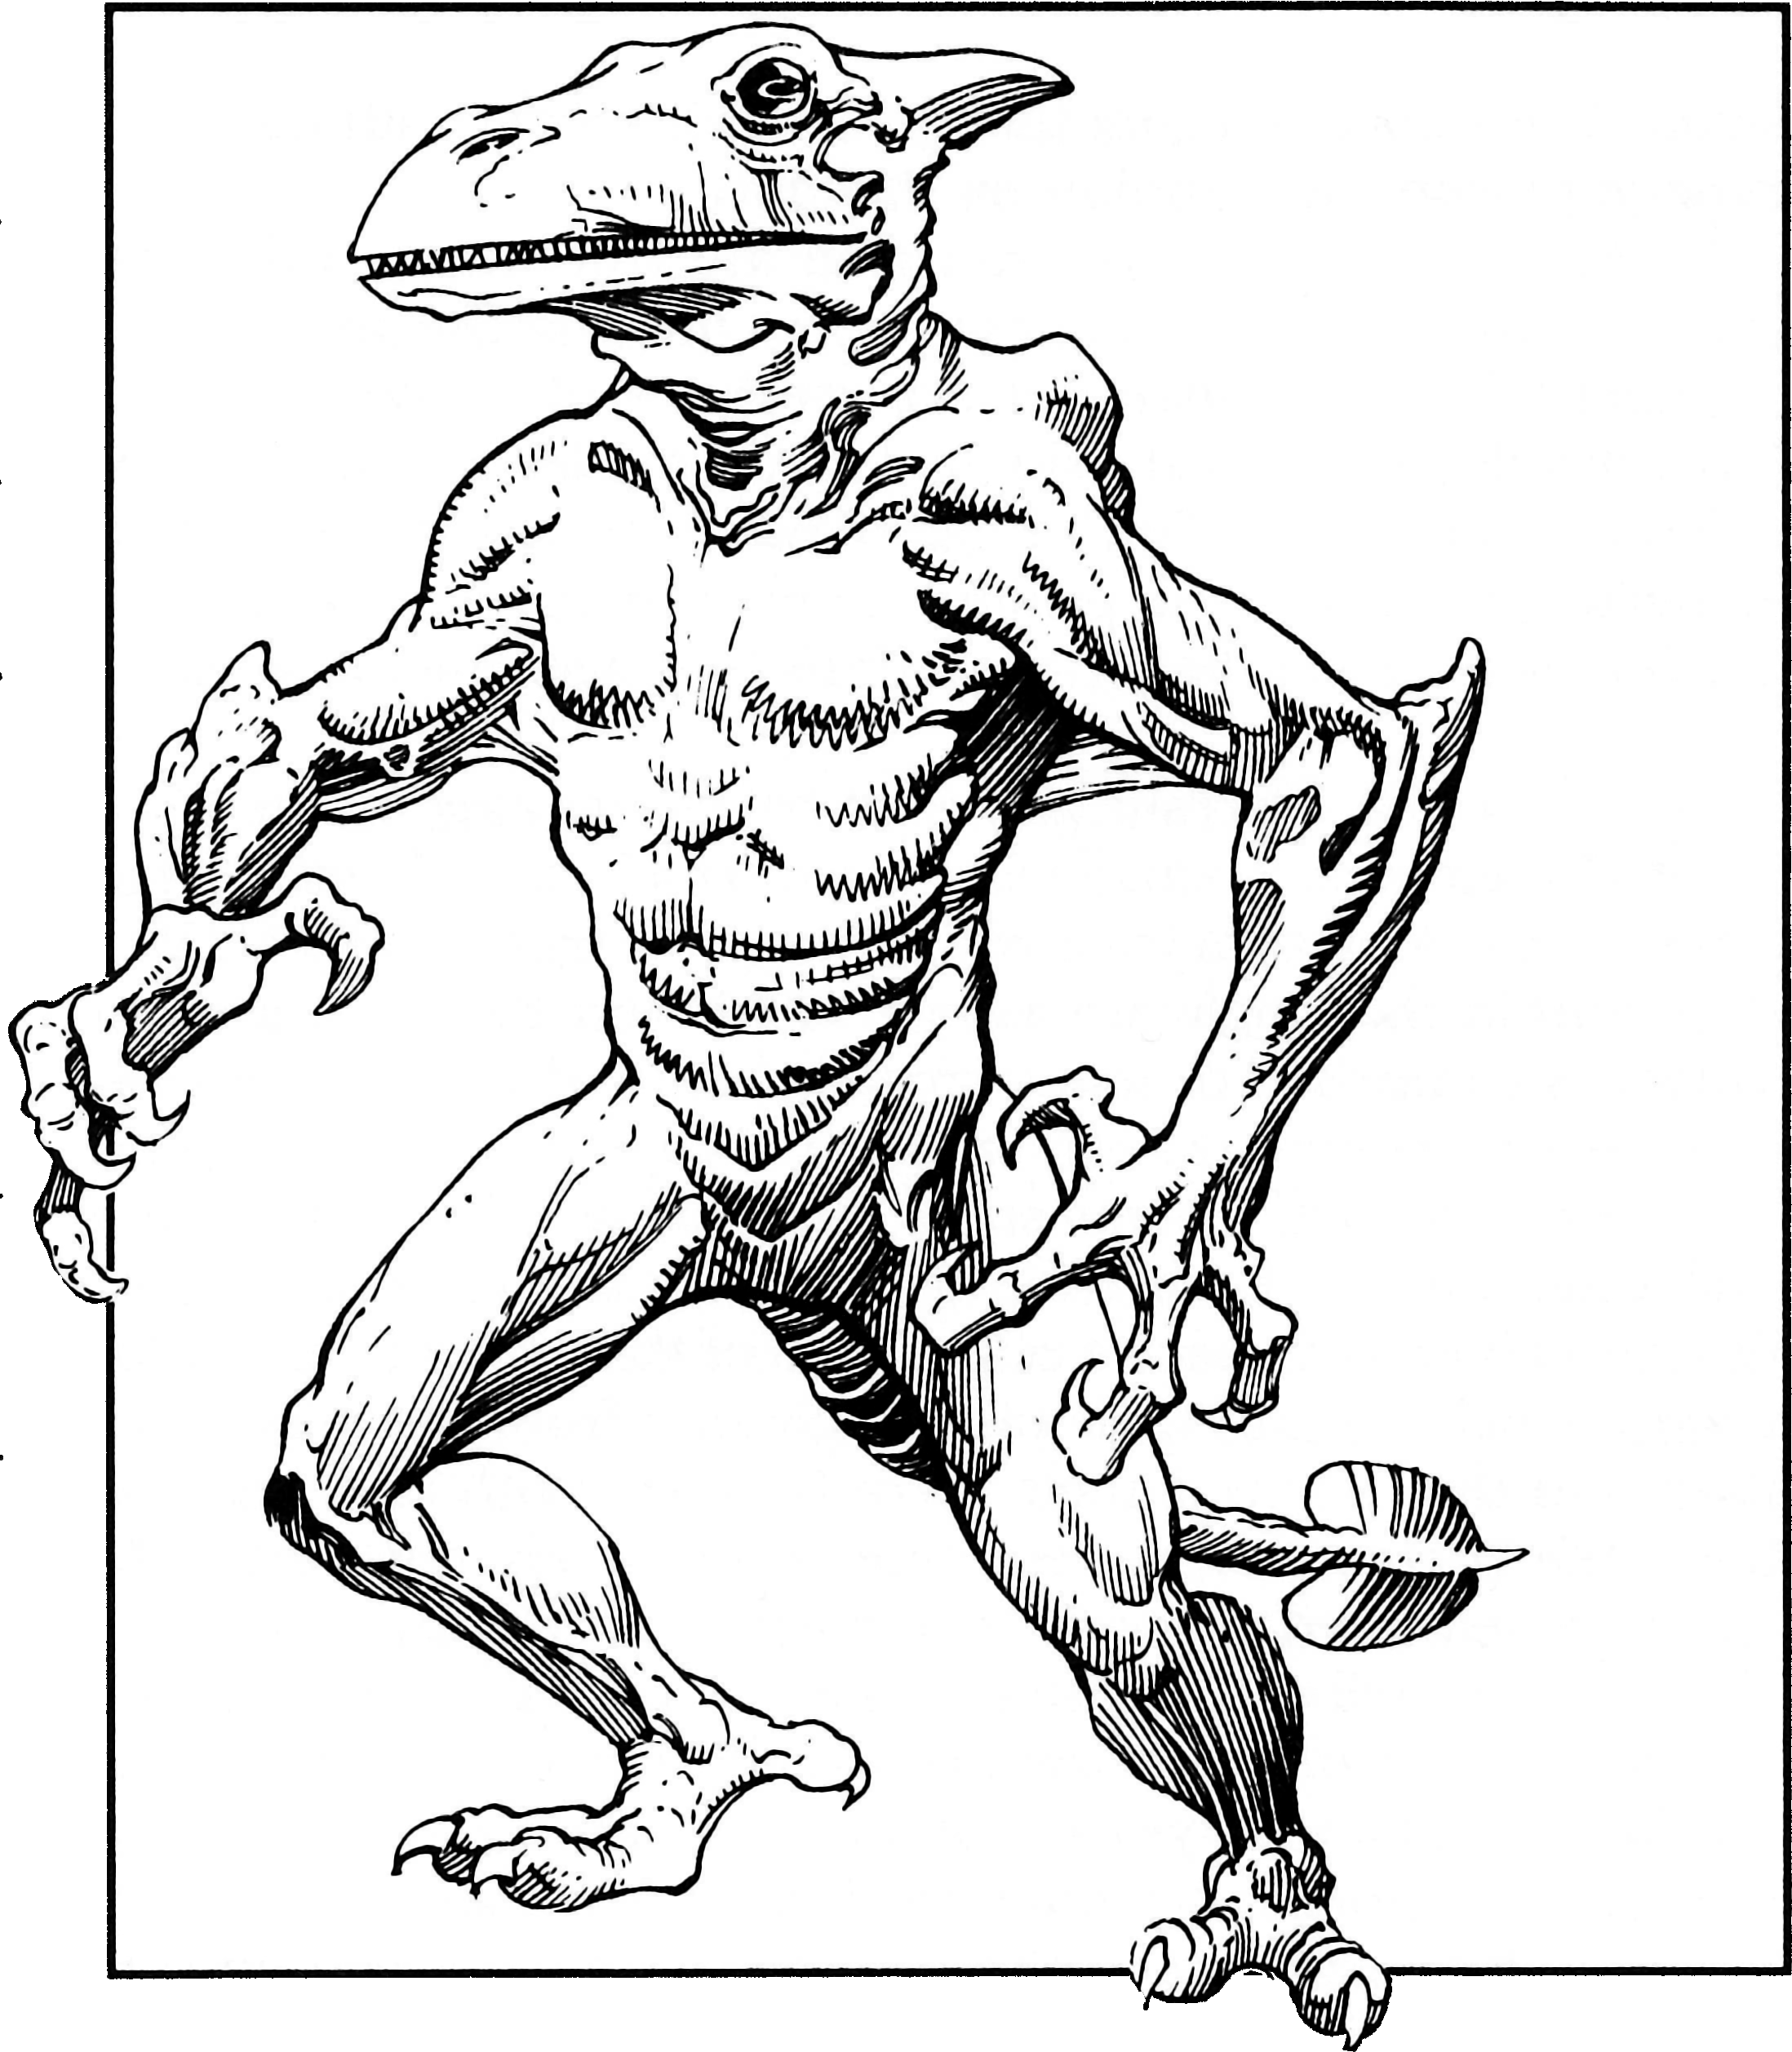
\includegraphics[width=\columnwidth]{images/pterran-1.png}
\WOTC
\end{figure}

\subsubsection{Pterran Society}
Pterran society is based largely on ceremony and celebrations. An area is set aside in the center of each village for ceremonies. Pterrans revere the world of Athas as the Earth Mother, and believe themselves to be her favored children. Throughout the day, they engage in a number of ceremonies that give thanks to the Earth Mother. These are led by druids who play a very important role in pterran society.

% A pterran village is a collection of many smaller family dwellings. Pterrans always bear young in pairs.

At age 15 every pterran chooses a ``life path.'' The three main life paths are the path of the warrior, the path of the druid and the path of the psionicist, though lesser life paths exist as well. More pterrans follow the path of the warrior than any of the other paths, and become protectors of their villages as well as the tribe's weapon makers. Pterrans that choose the path of the druid provide an important role in the daily ceremonies to the Earth Mother. Fewer pterrans choose the path of the psionicist than the other two major paths, as psionics are viewed as outside of nature. Psionicists are viewed with suspicion by the rest of the tribe; however, they do provide valuable skills to the tribe and are often the tribe's negotiators when they meet outsiders.

Pterrans are omnivores. Much of their diet comes from hunting animals and raising crops. Kirre, id fiend, and flailer are all considered pterran delicacies.

\subsection{Pterran Racial Traits}
\begin{itemize*}
    \item $-2$ Dexterity, +2 Wisdom, +2 Charisma: Pterrans' strong confidence and keen instincts for others' motives make them keen diplomats, and when they take the path of the psion, powerful telepaths.
    \item Humanoid (psionic, reptilian): Pterrans are humanoid creatures with the psionic and reptilian subtypes.
    \item Medium: As Medium creatures, pterrans have no special bonuses or penalties due to size.
    \item Pterran base land speed is 9 meters.
    \item Poor Hearing: Pterrans have only slits for ears, and their hearing sense is diminished. Pterrans suffer a $-2$ penalty to \skill{Listen} checks.
    \item Natural Weaponry: Pterrans can use their natural weapons instead of fighting with crafted weapons if they so choose. A pterran can rake with their primary claw attack for 1d3 of damage for each claw, and they bite for 1d4 points of damage as a secondary attack.
    \item Psi-Like Ability: At will---\psionic{missive}. All pterrans are gifted from the day they hatch with the ability to communicate telepathically, but only with their fellow reptiles. Manifester level is equal to \onehalf Hit Dice (minimum 1st).
    \item Weapon Familiarity: Pterrans treak thanak as a martial weapon rather than as an exotic weapon. This weapon is more common among pterrans than among other races.
    \item Automatic Languages: Saurian. Bonus Languages: Common, Dwarven, Elven, Giant, Gith, Halfling, Kreen, and Yuan-ti. Pterran know the languages of the few intelligent creatures that live in the Hinterlands.
    % \item Life Path: A pterran's life path determines his favored class. Those following the Path of the Druid have druid as a favored class; the Path of the Mind gives psion as a favored class, while the Path of the Warrior gives ranger as a favored class. A Pterran chooses a life path upon coming of age, and the path cannot be changed once chosen at character creation time.
    \item Favored Class: Druid.
\end{itemize*}